\section{Unauthenticated user}
\subsection{Signing up}
If you wish to sign up to \textit{EmporioLambda}, access any page of the website. In the header\textsubscript{G} section of the page you'll see a button with the text 'Register / Sign in'. Clicking it will redirect you to the login page.

\begin{figure}[H]
\centering
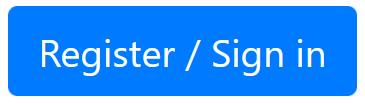
\includegraphics[scale=0.6]{res/Immagini/RegisterSigninButton}
\caption{Registration and sign in button}
\end{figure}

To proceed with the sign up procedure you will then have to click the 'Sign up' text. In the following picture, it is highlighted in red.

\begin{figure}[H]
\centering
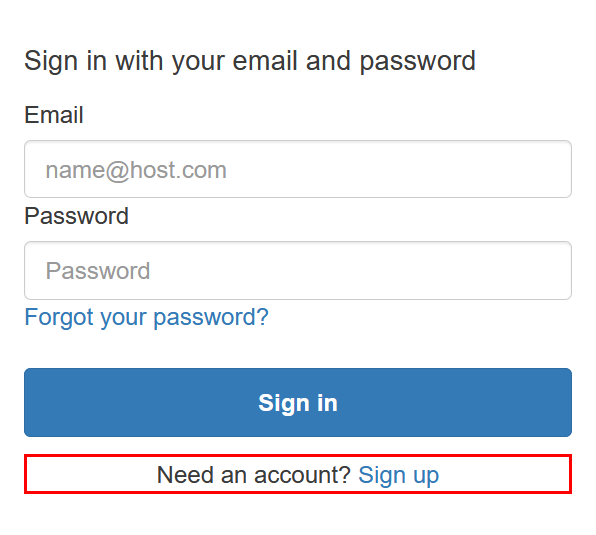
\includegraphics[scale=0.6]{res/Immagini/RegisterSigninForm}
\caption{Login form}
\end{figure}

You will then find yourself on a page with a form to insert your data. Every field is mandatory, and the system will not let you continue unless there is all the necessary data. 

The password field must contain a lower case letter, an upper case letter, a special character, a number and has to be at least 8 characters long.

\begin{figure}[H]
\centering
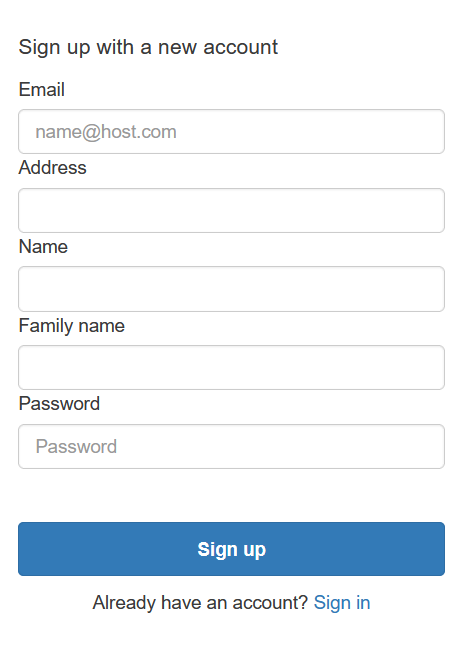
\includegraphics[scale=0.6]{res/Immagini/RegisterForm}
\caption{Sign up form}
\end{figure}

After compiling every field and clicking on the 'Sign up' button, you will see a page asking for a confirmation code. You will receive this code by email, on the address you specified in the last step. After inserting the code and clicking on the 'Confirm Account' button, you will have successfully completed the sign up procedure. You will therefore be redirected to the homepage, already signed in.

If, after waiting a few minutes, you still haven't received your confirmation code, you can try clicking on the 'Resend it' text to send it again.

\begin{figure}[H]
\centering
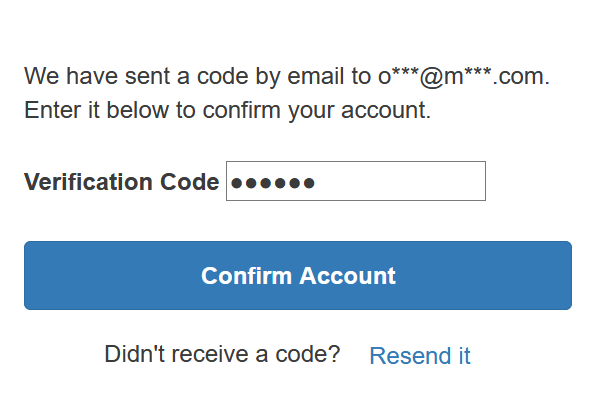
\includegraphics[scale=0.6]{res/Immagini/RegisterCode}
\caption{Confirmation code form}
\end{figure}

\subsubsection{Sign up error}
If any error happens during the registration procedure, you will be redirected to the previous section with an error message describing what the problem is. If the message isn't self explanatory, please refer to section 6 issue reporting.

\begin{figure}[H]
\centering
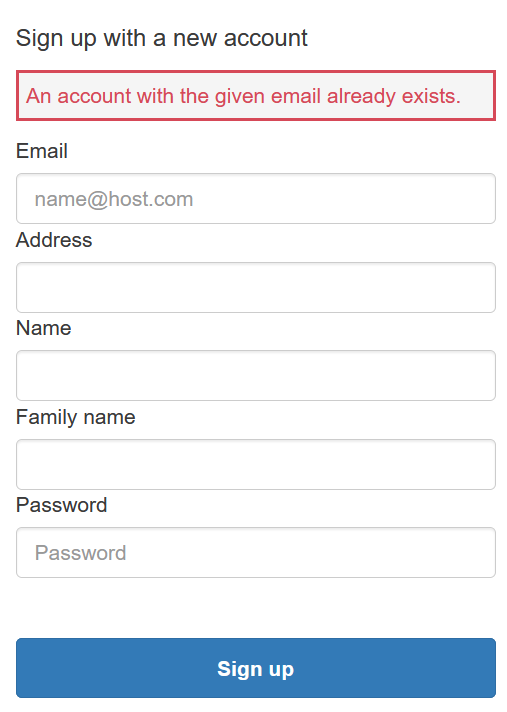
\includegraphics[scale=0.6]{res/Immagini/RegisterError}
\caption{Sign up error example: the email address is already in use}
\end{figure}

\subsection{Signing in}
In order to sign in to \textit{EmporioLambda}, an account is needed. If an account hasn't been created yet, refer to section 2.1 Signing up.

To sign in, access any page of the website. In the header\textsubscript{G} section of the page you'll see a button with the text 'Register / Sign in'. Clicking it will redirect you to the login page.

\begin{figure}[H]
\centering
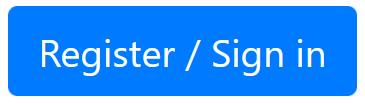
\includegraphics[scale=0.6]{res/Immagini/RegisterSigninButton}
\caption{Registration and sign in button}
\end{figure}

To proceed with the sign in procedure you will then have to insert your data in the sign in form. After compiling the form, click on the 'Sign in' button. If the email and password were correct, you will be redirected to the homepage of the website, successfully logged in.

\begin{figure}[H]
\centering
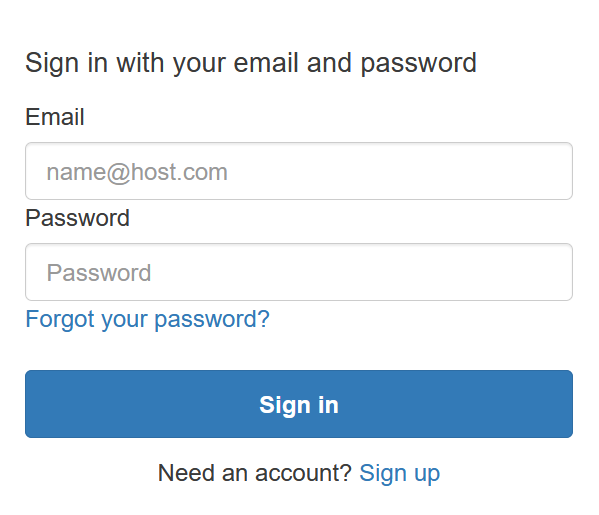
\includegraphics[scale=0.6]{res/Immagini/SigninForm}
\caption{Sign in form}
\end{figure}

\subsubsection{Forgotten password}
If you forgot your login password, click on the 'Forgot your password?' text. You will then have to insert your account's email and click on the 'Reset my password' button in order to continue.

\begin{figure}[H]
\centering
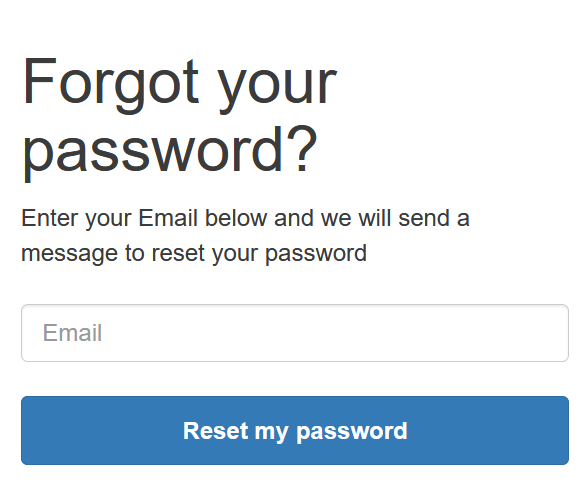
\includegraphics[scale=0.6]{res/Immagini/ResetPassword}
\caption{Forgot your password page}
\end{figure}

You will then have to fill a form with your new password. You will also receive a confirmation code by email, on the address you specified in the last step. This code will also have to be inserted in the form in order to reset your password.

Once the form is filled, click on the 'Change Password' button to reset your password. You will then be redirected to the login form, with your password updated.

\begin{figure}[H]
\centering
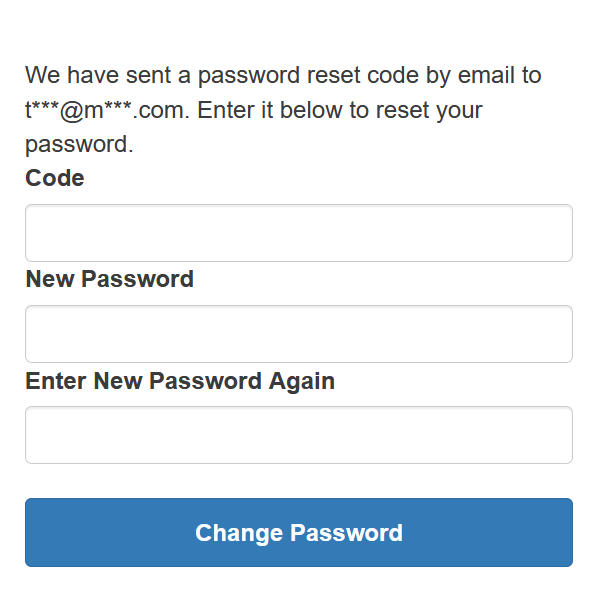
\includegraphics[scale=0.6]{res/Immagini/ResetPasswordForm}
\caption{Forgot your password page}
\end{figure}

\subsubsection{Sign in error}
If any error occurs during the login procedure, you will be redirected to the previous section with an error message describing what the problem is. If the message isn't self explanatory, please refer to section 6 issue reporting.

\begin{figure}[H]
\centering
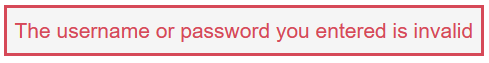
\includegraphics[scale=0.6]{res/Immagini/SigninError}
\caption{Example of a sign in error: the email or password were invalid}
\end{figure}

\subsection{Browsing by category}
To browse the products by category, access the homepage of the website by clicking on the 'Home' link in the header of the website. You will then see a list of all the product categories in the system.

\begin{figure}[H]
\centering
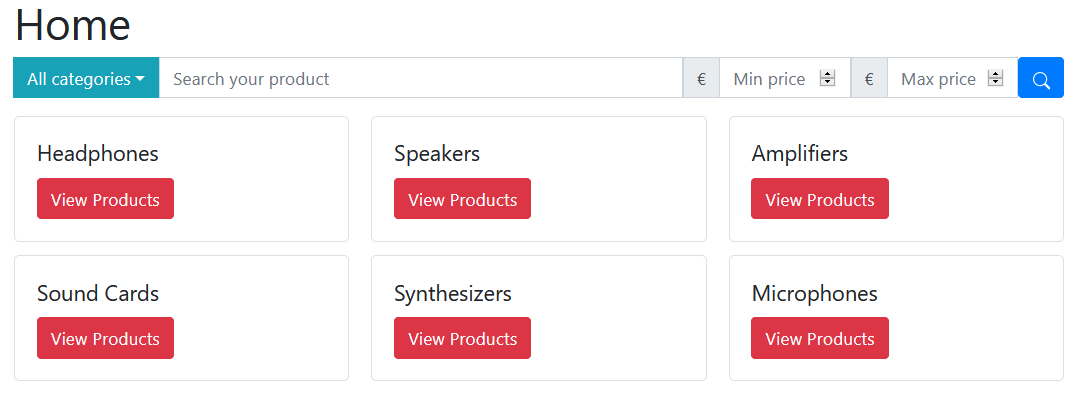
\includegraphics[scale=0.6]{res/Immagini/CategoryList}
\caption{Example of a homepage with a list of categories}
\end{figure}

To view the products in a category, click on the 'View Products' button. You will then be presented with a list of the products of the desired category.

\begin{figure}[H]
\centering
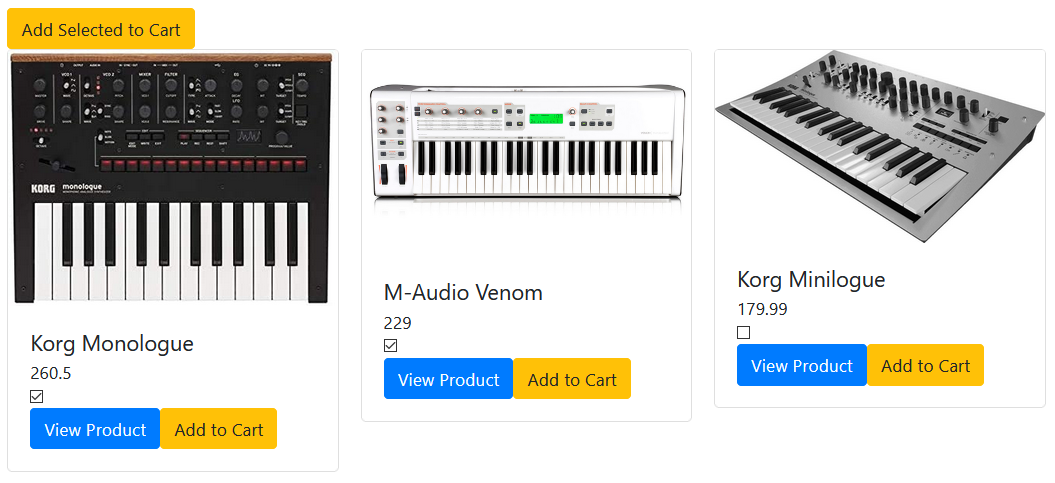
\includegraphics[scale=0.6]{res/Immagini/CategoryPage}
\caption{Example of a category page with a list of products}
\end{figure}

\subsection{Accessing a product page}
To access a product page, browse to a category page and click on the 'View Product' button. This will lead you to a section of the website that contains all of the details regarding a specific product. 

\begin{figure}[H]
\centering
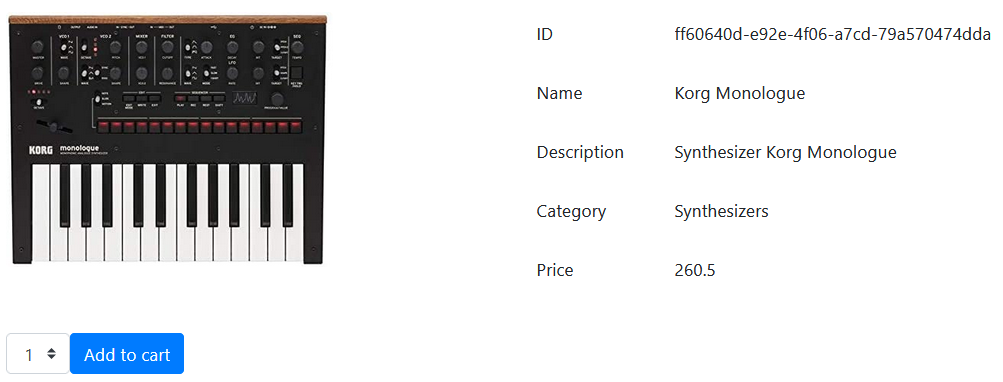
\includegraphics[scale=0.6]{res/Immagini/ProductPage}
\caption{Example of a product page}
\end{figure}

\subsection{Adding products to the cart}
In order to add a product to your cart, you must first browse to a category or a product page.

In a category page, to add the listed products individually, click on the 'Add to Cart' button. To add multiple products at the same time, click on the checkbox under all the products you wish to add to the cart and then click the 'Add Selected to Cart' button.

In a product page, select the number of items you want to add to your cart and click the 'Add to cart' button.

\subsection{Searching and filtering products}
In \textit{EmporioLambda} you can search for products by name and filter them by price and category. To do so, access the homepage, a category page or a product page.

\begin{figure}[H]
\centering
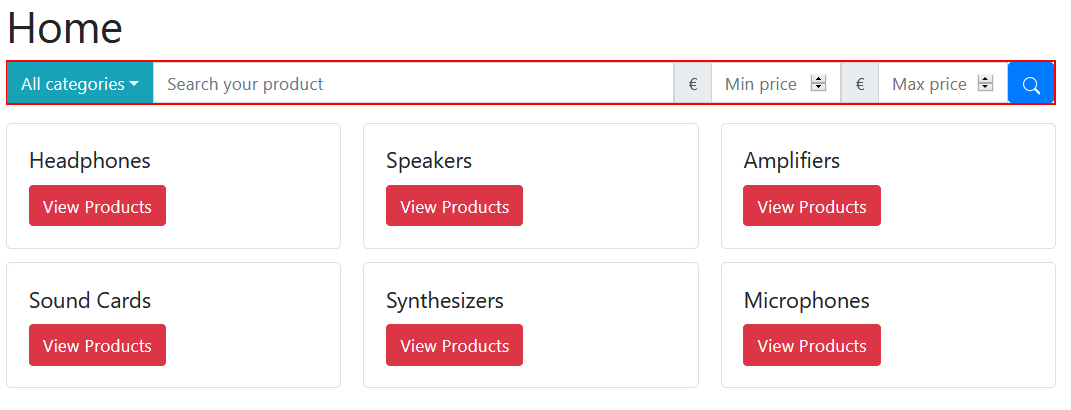
\includegraphics[scale=0.6]{res/Immagini/SearchFilterBar}
\caption{Search and filter bar}
\end{figure}

You will see a horizontal bar with various options for querying products.

\begin{itemize}
\item To filter by the product's category, click on the first element in the search bar. It will open a dropdown menu with a list of all the available categories;
\item To search for the product's name, enter your search query in the textbox that says 'Search for your product';
\item To filter by a price range, enter the maximum price, the minimum price or both in the related fields.
\end{itemize}

To send the search or filter query and retrieve the products that match it, click on the rightmost button in the searchbar. The text 'No product found' will be shown if no products match your request.

\subsection{Managing the cart}
To access and manage your cart, click on the 'Cart' link in the header section of the website. If you never added any products, you will see the text 'Your cart is empty'. Otherwise, you will see a list of the items you previously added to the cart.

\begin{figure}[H]
\centering
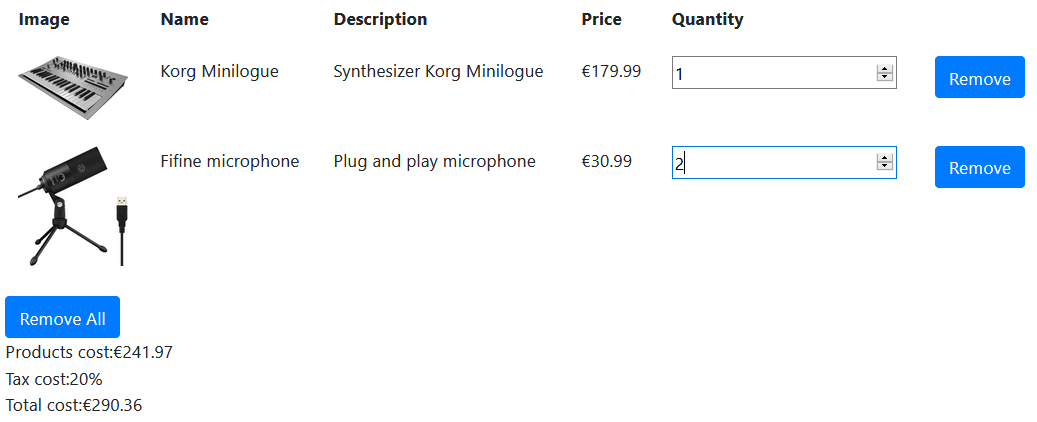
\includegraphics[scale=0.6]{res/Immagini/CartPage}
\caption{Example of a cart page}
\end{figure}

For each item you will see an image, the name, a description, the price and the quantity of items you intend to purchase.

To edit the quantity, either overwrite the number in the textbox or use the two arrows at the right of it. 

To remove an item, click on the 'Remove' button next to it. 

To remove all the items in the cart, click the 'Remove All' button.

At the bottom of the screen, you will see the product cost with and without the tax applied.